%!TEX root = ../thesis.tex

\chapter{Characterising SDE linearisations: the numerics}\label{ch:linear_numerics}
In this chapter, we provide numerical validation of the results in \Cref{ch:linear_theory} on example stochastic differential equations.
A majority of the context this chapter again appears in the submitted article \citep{BlakeEtAl_2023_ConvergenceStochasticDifferential}.
The overview in \Cref{sec:mazzoni} of an algorithm for efficiently solving the mean-covariance equations for the linearisation approximation does not appear in the submitted article.
\Cref{sec:comput_s2} provides an initial and heuristic comparison between the stochastic sensitivity and finite-time Lyapunov fields, which also does not appear in the submitted article.

\section{Mazzoni's method}\label{sec:mazzoni}
\td{Update equation references! Relate to stuff in the paper, not the later chapter!!}
An important consideration  when solving \cref{eqn:gauss_de} numerically is that \(\Pi_t\) represents a covariance matrix and must remain symmetric and positive semi-definite.
However, many standard numerical ODE schemes do not take this into account, so a specialised scheme is required.
Similar equations of the form \cref{eqn:gauss_de} (although often without explicit dependence on both time and the state in the \(\sigma\) term) are solved numerically in other applications, notably when implementing the extended Kalman filter \citep{Jazwinski_2014_StochasticProcessesFiltering, KulikovaKulikov_2014_AdaptiveODESolvers}.
\citet{KulikovaKulikov_2014_AdaptiveODESolvers} identify that that the two most significant sources of numerical error when solving \cref{eqn:gauss_de} are a) the estimate of the covariance matrix \(\Sigma_s^t\) violating the requirement of positive semi-definiteness, and b) local error propagation in the state equation.
Moreover, a computationally efficient algorithm is critical to ensure that our approximate methods have an advantage over bulk Monte-Carlo simulation.

\citet{Mazzoni_2008_ComputationalAspectsContinuous} proposes an efficient hybrid method for solving \cref{eqn:gauss_de} which addresses both difficulties a) and b) and takes advantage of the availability of \(\nabla u\).
This method, which we shall term the Mazzoni method, combines a Taylor-Heun approximation for \cref{eqn:gauss_mean_de} and a Gauss-Legendre step for \cref{eqn:gauss_cov_de}.
With a step size of \(\delta t\), integration for both the state variable and the covariance matrix are convergent with order \(\mathcal{O}\!\left(\delta t^2\right)\).
Moreover, \citet{Mazzoni_2008_ComputationalAspectsContinuous} shows through numerical simulations that the algorithm is computationally efficient when compared to alternatives with moderate precision.
We therefore employ the Mazzoni method for all subsequent computations of the linearisation solution.

The Mazzoni algorithm is summarised in the following.
Further details on the derivation of these equations is available in the original article \citep{Mazzoni_2008_ComputationalAspectsContinuous}.
The Taylor-Heun formula for the update of the state over the interval \([t, t + \delta t]\) is
\begin{subequations}\label{eqn:mazzoni_update}
	\begin{equation}
		w_{t + \delta t} \approx w_t + \left(I - \frac{\delta t}{2}\nabla u\left(w_t, t\right)\right)^{-1}.
		\label{eqn:mazzoni_state_update}
	\end{equation}
	The Gauss-Legendre update of the covariance matrix is
	\begin{equation}
		\Pi_{t + \delta t} \approx M_\tau \Pi_t M_\tau^{\T} + \delta t K_\tau \sigma\left(w_\tau,\, t + \frac{\delta t}{2}\right)\sigma\left(w_\tau,\, t + \frac{\delta t}{2}\right)^{\T} K_\tau^{\T},
		\label{eqn:mazzoni_cov_update}
	\end{equation}
	where
	\begin{align}
		w_\tau & = \frac12\left(w_t + w_{t + \delta t} - \frac{\delta t^2}{4}\nabla u\left(w_t, \, t\right) u\left(w_t, \, t\right)\right) \label{eqn:mazzoni_cov_terms1} \\
		K_\tau & = \left[I - \frac{\delta t}{2}\nabla u\left(w_\tau,\, t + \frac{\delta t}{2}\right)\right]^{-1}                                                          \\
		M_\tau & = K_\tau \left[I + \frac{\delta t}{2}\nabla u\left(w_\tau,\, t + \frac{\delta t}{2}\right)\right] \label{eqn:mazzoni_cov_terms3}.
	\end{align}
	The vector \(w_\tau\) serves as an interpolation between \(w_t\) and \(w_{t + \delta t}\) for the state at time \(t + \delta t / 2\), which is used to provide a more accurate approximation of the covariance matrix.
	\citet{Mazzoni_2008_ComputationalAspectsContinuous} also provides the option of an adaptive time step to fix the numerical precision while ensuring a computationally efficient algorithm.
	The step size is adjusted by monitoring the error in the estimation of the state variable, aiming to maintain a specified tolerance level \(\gamma > 0\).
	Given the error vector \(\mathcal{E}\) for each component of the state approximation, the maximum total-relative error is
	\begin{equation}\label{eqn:mazzoni_e}
		\hat{\gamma} = \max_{i = 1,\dots,n}\frac{\abs{\mathcal{E}^{(i)}}}{\abs{w_{t + \delta t}^{(i)}} + 1}
	\end{equation}
	where \(\mathcal{E}^{(i)}\) and \(w_{t + \delta t}^{(i)}\) denote the respective \(i\)th elements of \(\mathcal{E}\) and \(w_{t + \delta t}\).
	The resulting adjustment factor for the time step is
	\begin{equation}\label{eqn:mazzoni_step}
		\delta t_{\mathrm{new}} = \beta \delta t \sqrt{\frac{\gamma}{\hat{\gamma}}}.
	\end{equation}
	The factor \(\beta\) is a control parameter inserted to avoid frequent recalculations of the step size, and is specified prior.
	\citet{Mazzoni_2008_ComputationalAspectsContinuous} suggests setting \(\beta = 0.8\).
	By again taking advantage of the availability of the Jacobian \(\nabla u\), the error vector is approximated as
	\begin{equation}\label{eqn:mazzoni_err}
		\mathcal{E} \approx \frac{\delta t^2}{2}\left[\frac{1}{3\delta t}\left(\nabla u\!\left(w_{t + \delta t}, t + \delta t\right) - \nabla u\!\left(w_t, t\right)\right) - \frac{1}{6}\nabla u\!\left(w_t, t\right)^2\right] u\!\left(w_t, t\right).
	\end{equation}
\end{subequations}
The set of equations \cref{eqn:mazzoni_update} describe the Mazzoni algorithm, and in \Cref{fig:mazzoni_alg} we summarise the full algorithm with an adaptive step size.

\begin{figure}
	\begin{center}

		\begin{tikzpicture}[node distance=70pt]
			\tikzstyle{arrow} = [->,>=stealth]

			\node (s) [rectangle, rounded corners, draw=black, align=center] {\textbf{Start} \\ Given \(s, T, x_s, \Sigma_s\) \\ Choose \(\delta t_{\mathrm{min}}, \beta, \gamma\)};

			\node (a) [rectangle, below of=s, draw=black, align=center, yshift=-10pt] {Set \(t_0 = s\) \\ Set \(w_{t_0} = x_s\) \\ Set \(\Pi_{t_0} = \Sigma_s\) Set \(\delta t = \delta t_{\mathrm{min}}\) \\ Set \(k = 0\)};
			\node (b) [rectangle, below of=a, draw=black, align=center, yshift=-20pt] {Set \(t_{k+1} = t_k + \delta t\) \\ Compute \(w_{t_{k+1}}\) with \cref{eqn:mazzoni_state_update} \\
				Compute \(e\) with \cref{eqn:mazzoni_e} \\ Set \(\delta t_{\mathrm{new}} = \max\left\{\delta t_{\mathrm{min}}, \beta \delta t \sqrt{\frac{\gamma}{\hat{\gamma}}}\right\}\)};

			\node (d) [diamond, below of=b, draw=black, align=center, yshift=-40pt] {\(\hat{\gamma} \leq \gamma\) or \\ \(\delta t \leq \delta t_{\mathrm{min}}\)?};
			\node (c) [rectangle, left of=d, draw=black, align=center, xshift=-75pt] {Set \(\delta_t = \delta_{\mathrm{new}}\)};

			\node (e) [rectangle, below of=d, draw=black, align=center, yshift=-20pt] {Compute \(\Pi_{t_{k+1}}\) with \crefrange{eqn:mazzoni_cov_terms1}{eqn:mazzoni_cov_terms3} \\ Set \(k = k + 1\)};

			\node (f) [diamond, below of=e, draw=black, align=center] {\(t_k = T\)?};

			\node (g) [rectangle, rounded corners, left of=f, draw=black, align = center, xshift = -30pt] {\textbf{Stop}};
			\node (h) [rectangle, right of=f, draw=black, align = center, xshift = 75pt] {\(\delta t = \min\left\{\delta t_{\mathrm{new}}, T - t_k\right\}\)};

			\draw [arrow] (s) -- (a);

			\draw [arrow] (a) -- (b);
			\draw [arrow] (b) -- (d);

			\draw [arrow] (d) -- node[anchor=south] {no} (c);
			\draw [arrow] (d) -- node[anchor=east] {yes} (e);

			\draw [arrow] (c) |- (b);

			\draw [arrow] (e) -- (f);

			\draw [arrow] (f) -- node[anchor=south] {yes} (g);
			\draw [arrow] (f) -- node[anchor=south] {no} (h);

			\draw [arrow] (h) |- (b);
		\end{tikzpicture}
		\caption{A flowchart of the Mazzoni algorithm with adaptive time stepping.
			Recreated from Figure 2 of \citet{Mazzoni_2008_ComputationalAspectsContinuous}.}
		\label{fig:mazzoni_alg}
	\end{center}
\end{figure}




\section{Numerical validation \& examples}\label{sec:numerics}
This section will validate the theory presented in \Cref{sec:theory,sec:theory_s2}, by considering three example SDEs each leading to a different form of the strong error bound \cref{eqn:main_ineq}.
For each example, we first demonstrate heuristically that the solution converges to the limiting distribution described by \Cref{thm:limit_sol}, and then verify the error bound in \Cref{thm:main} directly by considering a range of values for the noise scale \(\epsilon\) and initial condition uncertainty \(\delta_r\).
We demonstrate numerically the form of the bound on the linearisation error predicted by \Cref{thm:main} is sharp, in the sense that estimates of the error scale exactly with the initial uncertainty \(\delta_r\) and ongoing uncertainty \(\epsilon\) as predicted.


All simulations in this section were generated using the Julia programming language \citep{BezansonEtAl_2017_JuliaFreshApproach}, with the implementations of numerical ODE and SDE solvers provided by the DifferentialEquations.jl package \citep{RackauckasNie_2017_DifferentialEquationsJlPerformant}.
The code is available at \href{https://github.com/liamblake/explicit-characterisation-sde-linearisation}{github.com/liamblake/explicit-characterisation-sde-linearisation}.




\subsection{Nonlinear dynamics, additive noise}\label{sec:numerics_nonlinear}
Consider the following SDE in 1D;
\begin{equation}\label{eqn:sine_sde}
	\dif y_t^{(\epsilon)} = \sin\!\left(y_t^{(\epsilon)}\right)\dif t + \epsilon \dif W_t.
\end{equation}
The deterministic system corresponding to \cref{eqn:sine_sde} has solution
\[
	F_0^t\!\left(x_0\right) = 2\arctan\left(e^{-t}\tan\left(\frac{x_0}{2}\right)\right).
\]
Further details of this example, including computation of the derivatives required in the linearisation, are provided in the supplementary material.

To explore the impact of initial condition uncertainty, we consider the univariate Gaussian initial condition \(y_0 = x \sim \Gauss{\mu, \rho^2}\), where the mean \(\mu\) is specified and the standard deviation \(\rho\) is a non-negative scaling parameter.
We linearise \cref{eqn:sine_sde} about the deterministic trajectory \(F_0^t\!\left(\mu\right)\) originating from the mean, that is, \(\mu\) is the chosen reference point.
This ensures that for any \(r \geq 0\)
\begin{equation}\label{eqn:num_gauss_init}
	\delta_r^r = \avg{\abs{x - \mu}^r} = M_r \rho^r.
\end{equation}
where \(M_r\) is as defined in \cref{eqn:gauss_dist_bound}.
This property of the univariate Gaussian distribution allows us to easily control the uncertainty in the initial condition and verify the bounds; by sending the parameter \(\rho\) to zero we ensure that \(\delta_r\) approaches zero also.

The linearised equation is then
\begin{equation}
	\dif l_t^{(\epsilon)} = \left[F_0^t\!\left(\mu\right) + \cos\!\left(F_0^t\!\left(\mu\right)\right)\left(l_t^{(\epsilon)} - F_0^t\!\left(\mu\right)\right)\right]\dif t + \epsilon \dif W_t, \quad l_0^{(\epsilon)} \isGauss{\mu, \rho^2}.
	\label{eqn:sine_linear}
\end{equation}
and the solution follows a Gaussian distribution, specifically
\begin{equation}\label{eqn:num_linear_sol}
	l_t^{(\epsilon)} \isGauss{F_0^t\!\left(\mu\right), \, \rho^2\nabla F_0^t\!\left(\mu\right)^2 + \epsilon^2\Sigma_0^t\!\left(\mu\right)}.
\end{equation}
where \(\Sigma_0^t\!\left(\mu\right)\) is computed by solving \cref{eqn:pi_ode} numerically subject to a zero initial condition.

In this example, we take \(\mu_0 = 0.5\) and consider the solutions of \cref{eqn:sine_sde} and \cref{eqn:sine_linear} at time \(t = 1.5\).
We generate accurate samples of \cref{eqn:sine_sde} and \cref{eqn:sine_linear} jointly (i.e. using the same numerical realisations of the Wiener process \(W_t\)) using the stochastic Runge-Kutta scheme SRI \citep{Rossler_2010_RungeKuttaMethodsStrong} with an adaptive step size \citep{RackauckasNie_2017_AdaptiveMethodsStochastic}.

\begin{figure}
	\begin{center}
		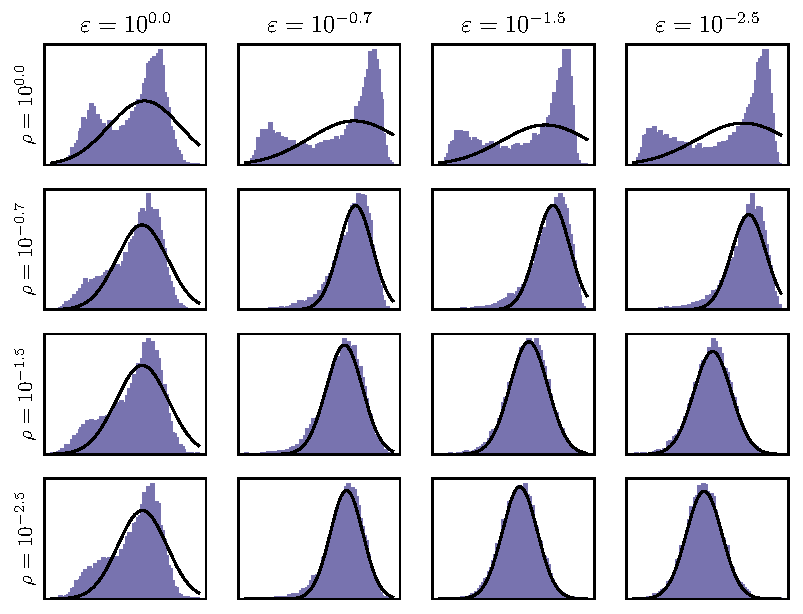
\includegraphics[width=\textwidth]{chp04_paper_numerics/figures/sine/selected_hists.pdf}
		\caption{Histograms of stochastic samples of \cref{eqn:sine_sde}, subject to the Gaussian initial condition \cref{eqn:num_gauss_init}, for varying initial uncertainty scale \(\rho\) and ongoing uncertainty scale \(\epsilon\).
			The distribution of the corresponding solution \cref{eqn:num_linear_sol} to the linearised equation is overlaid in black.}
		\label{fig:sine_hists}
	\end{center}
\end{figure}

In \Cref{fig:sine_hists}, we show histograms of \(N = 10000\) samples of the solution to nonlinear SDE \cref{eqn:sine_sde} and the corresponding probability density function of the linearised solution \cref{eqn:num_linear_sol}, for different combinations of \(\epsilon\) and \(\rho\).
Even when the ongoing noise is small, the nonlinearity of the drift term means that a large initial uncertainty results in a non-Gaussian distribution.
However, in situations where both the initial and ongoing uncertainties are small, the Gaussian solution to the linearised equation provides a reasonable approximation.
In the limit of both small initial (\(\rho \to 0\)) and small ongoing (\(\epsilon \to 0\)) uncertainty (towards the bottom right), we see that the distribution of the samples approach the Gaussian density of the linearisation solution, matching the understanding that the linearisation approximation is ``reasonable'' for small noise regimes.

Since the drift term is nonlinear and the noise is additive in \cref{eqn:sine_sde}, the bound predicted by \Cref{thm:main} has the form
\[
	\avg{\norm{y_t^{(\epsilon)} - l_t^{(\epsilon)}}^r} \leq D_1\!\left(r,t, K_{\nabla u}, K_\sigma\right)\epsilon^{2r} + M_{2r}D_2\!\left(r,t, K_{\nabla u}\right)\rho^{2r}.
\]
where we have taken \(K_{\nabla\nabla u} = 1\) and \(K_{\nabla\sigma} = 0\).
To numerically validate this bound under the Gaussian initial condition \cref{eqn:num_gauss_init}, define for \(r \geq 1\) the error measure
\begin{equation}
	E_r\!\left(\epsilon, \rho\right) \coloneqq \frac{1}{N}\sum_{i=1}^N{\norm{\hat{y}_{i}^{(\epsilon)} - \hat{l}_i^{(\epsilon)}}^r},
	\label{eqn:strong_err_mc_estimate}
\end{equation}
which is a Monte-Carlo estimator of the right-hand side of \cref{eqn:main_ineq}, where \(\hat{y}_1^{(\epsilon)},\dotsc, \hat{y}_N^{(\epsilon)}\) and \(\hat{l}_1^{(\epsilon)},\dotsc, \hat{l}_N^{(\epsilon)}\) are \(N\) numerical samples of the solutions to SDE \cref{eqn:sde_y} and the linearisation \cref{eqn:linear_sde_inform} respectively.

We directly validate the \emph{form} of the error bound (as a function of \(\epsilon\) and \(\rho\)) in \Cref{fig:sine_delta_eps_lines}, by computing \(E_1\) using samples for each pair of \(\epsilon\) and \(\rho\) values.
In \Cref{fig:sine_eps_lines}, we demonstrate the relationship between \(E_1\) and the ongoing uncertainty \(\epsilon\) for several different fixed values of \(\rho\), each corresponding to a different colour.
A least squares estimate of a line of best fit of the form \(E_1 = \beta_0 + \beta_1 \epsilon^2 \), for fixed coefficients \(\beta_0\) and \(\beta_1\), is fitted to the observed errors (in untransformed space) to verify the scaling of our bound in \Cref{thm:main}.
We see that the line of best fit accurately matches the observed values of \(E_1\), verifying that \(E_1\) is in fact scaling with \(\epsilon^2\) as predicted.
\Cref{fig:sine_delta_lines} provides a similar demonstration between \(E_1\) and the initial uncertainty \(\rho\), where now each colour corresponds to a different fixed value of \(\epsilon\).
We again fit lines of the form \(E_1 = \beta_0 + \beta_1 \rho^2\) to verify the scaling of the bound, and see that the lines match the observed values of \(E_2\).
Thus, we have also validated that \(E_1\) scales with \(\rho^2\), as expected from \Cref{thm:main}.

\begin{figure}
	\begin{center}
		\begin{subfigure}{\textwidth}
			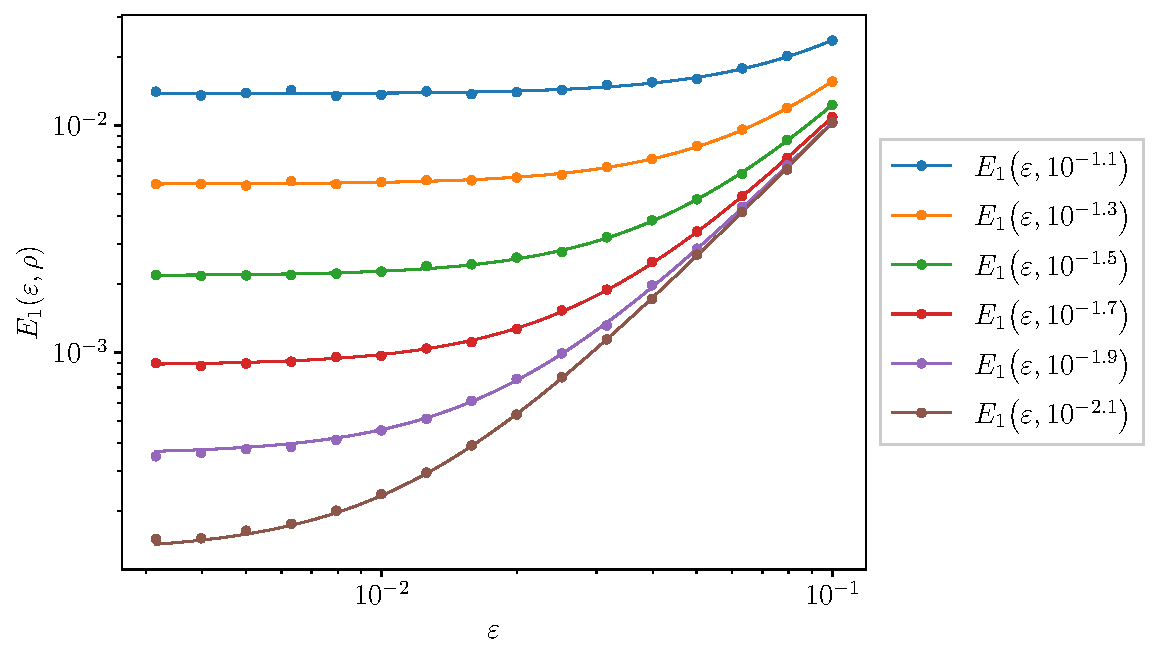
\includegraphics[width=\textwidth]{chp04_paper_numerics/figures/sine/str_err_eps_r_1.0_log.pdf}
			\caption{Estimates of the strong error (with \(r = 1\)) in linearising \cref{eqn:sine_sde} with \cref{eqn:sine_linear}, for varying ongoing uncertainty parameter \(\epsilon\).
				Each colour corresponds to a different value of the initial uncertainty parameter \(\rho\).
				A (least squares) line of best fit of the form \(\beta_0 + \beta_1 \epsilon^2\) is included in the corresponding colour.}
			\label{fig:sine_eps_lines}
		\end{subfigure}
		\begin{subfigure}{\textwidth}
			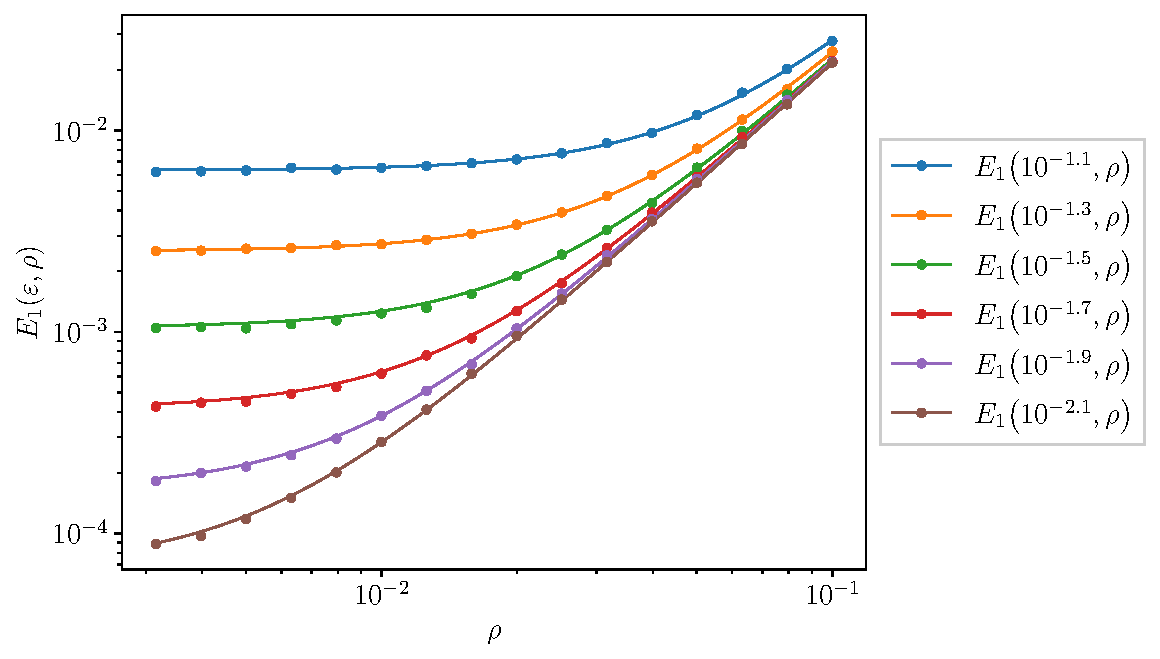
\includegraphics[width=\textwidth]{chp04_paper_numerics/figures/sine/str_err_rho_r_1.0_log.pdf}
			\caption{Estimates of the strong error (with \(r = 1\)) for varying initial uncertainty parameter \(\rho\).
				Each colour corresponds to a different value of the ongoing uncertainty parameter \(\epsilon\).
				A (least squares) line of best fit of the form \(\beta_0 + \beta_1 \rho^2\) is included in the corresponding colour.}
			\label{fig:sine_delta_lines}
		\end{subfigure}
		\caption{Validation of the theoretical bound predicted by \Cref{thm:main}, when \(r = 1\), on numerical realisations of the solution to the 1D example \cref{eqn:sine_sde}.}
		\label{fig:sine_delta_eps_lines}
	\end{center}
\end{figure}

\subsection{Linear dynamics, multiplicative noise}\label{sec:numerics_multiplicative}
Now consider the following SDE with multiplicative noise in 1D;
\begin{equation}
	\dif y_t^{(\epsilon)} = \frac12 y_t^{(\epsilon)}\dif t + \varepsilon \cos\!\left(y_t^{(\epsilon)}\right) \dif W_t.
	\label{eqn:1d_mult}
\end{equation}
The corresponding deterministic system is linear and has solution
\begin{equation}
	F_0^t\!\left(x_0\right) = \exp\!\left(\frac{t}{2}\right) x_0,
	\label{eqn:1d_mult_det_sol}
\end{equation}
with additional details provided in the supplementary materials.
As with the previous example in \Cref{sec:numerics_nonlinear}, we take the Gaussian initial condition \cref{eqn:num_gauss_init} with variance \(\rho^2\) and linearised \cref{eqn:1d_mult} about the initial mean \(\mu\).
The linearised equation is then
\begin{equation}
	\dif l_t^{(\epsilon)} = \frac12 l_t^{(\epsilon)}\dif t + \epsilon \cos\!\left(\exp\left(\frac{t}{2}\right)\mu\right) \dif W_t, \quad l_0^{(\epsilon)} \sim \Gauss{\mu, \rho^2},
	\label{eqn:1d_mult_linear}
\end{equation}
with Gaussian solution \cref{eqn:num_linear_sol}.
We take the initial point \(\mu = 2\) and consider the solutions at time \(t = 1\).
To generate numerical realisations of the solutions to \cref{eqn:1d_mult} and \cref{eqn:1d_mult_linear} with the same realisations of \(W_t\), we use the same set-up as in the previous example.

In \Cref{fig:sine_hists}, we show histograms of \(N = 10000\) samples of the multiplicative noise SDE \cref{eqn:1d_mult} and the corresponding probability density function of the linearised solution, for different combinations of \(\epsilon\) and \(\rho\).
We again see that in the limit of both small initial and small ongoing uncertainty (towards the bottom right), we see that the distribution of the samples approach the Gaussian density of the linearisation solution.

\begin{figure}
	\begin{center}
		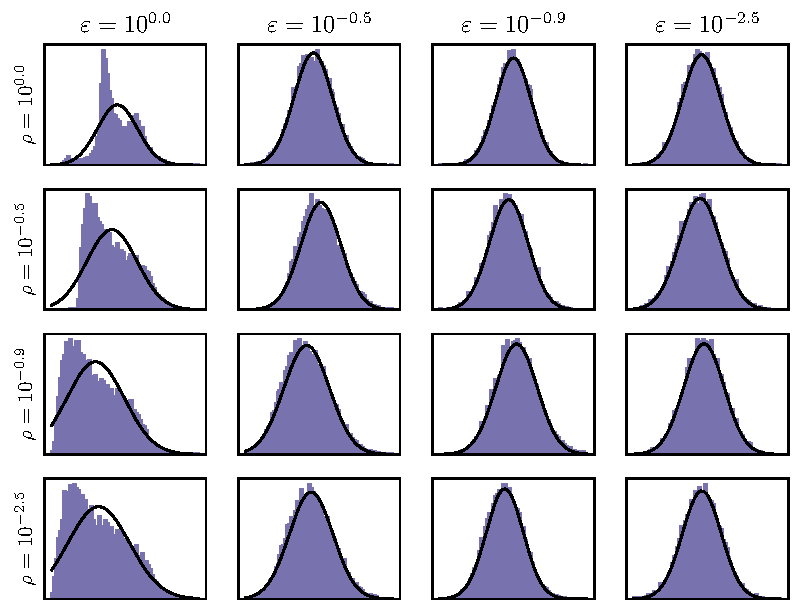
\includegraphics[width=\textwidth]{chp04_paper_numerics/figures/multiplicative/selected_hists.pdf}
		\caption{The same arrangement as \Cref{fig:sine_hists}, but for the 1D multiplicative noise SDE \cref{eqn:1d_mult}.}
		\label{fig:1d_mult_hists}
	\end{center}
\end{figure}

Since the drift term is linear and the noise multiplicative in \cref{eqn:1d_mult}, the bound predicted by \Cref{thm:main} has the form
\[
	\avg{\norm{y_t^{(\epsilon)} - l_t^{(\epsilon)}}^r} \leq D_1\!\left(r,t, K_{\nabla u}, K_\sigma\right)\epsilon^{2r} + M_{r}D_3\!\left(r,t, K_{\nabla u}\right)\epsilon^r\rho^{r},
\]
where we have \(K_{\nabla\nabla u} = 0\) and \(K_{\nabla\sigma} = 1\).
In \Cref{fig:multiplicative_delta_eps_lines}, we again validate the form of this bound (for \(r = 1\); results for additional values of \(r\) are provided in the supplementary material) by approximating the left-hand side with \(E_1\) computed from realisations of the solution to \cref{eqn:1d_mult} and the linearisation \cref{eqn:1d_mult_linear}.
For each fixed value of the initial uncertainty \(\rho\), in \Cref{fig:multiplicative_eps_lines}, we fit a line of best fit of the form \(\beta_1 \epsilon + \beta_2 \epsilon^2\) to validate that the strong error scales as predicted.
Similarly, in \Cref{fig:multiplicative_eps_lines} we fit a line of best fit of the form \(\beta_0 + \beta_1 \rho\) and confirm that the linearisation error follows this scaling.

\begin{figure}
	\begin{center}
		\begin{subfigure}{\textwidth}
			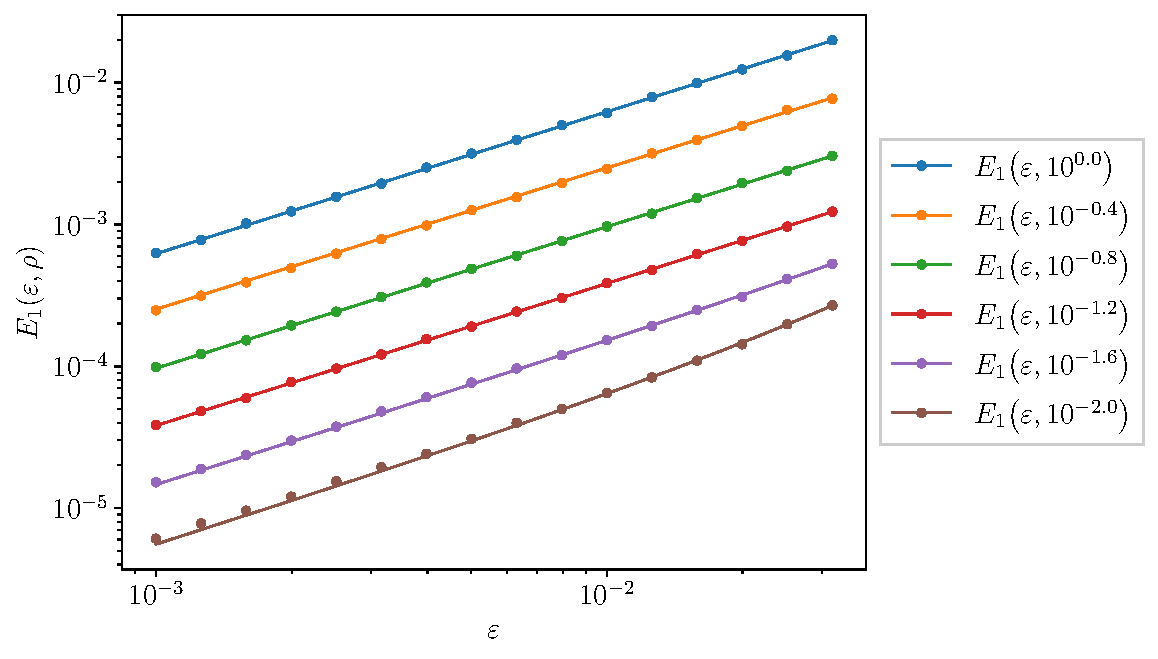
\includegraphics[width=\textwidth]{chp04_paper_numerics/figures/multiplicative/str_err_eps_r_1.0_log.pdf}
			\caption{Estimates of the strong order (with \(r = 1\)) for varying ongoing uncertainty parameter \(\epsilon\).
				Each colour corresponds to a different value of the initial uncertainty parameter \(\rho\).
				A (least squares) line of best fit of the form \(\beta_1 \epsilon + \beta_2 \epsilon^2\) is included in the corresponding colour.}
			\label{fig:multiplicative_eps_lines}
		\end{subfigure}
		\begin{subfigure}{\textwidth}
			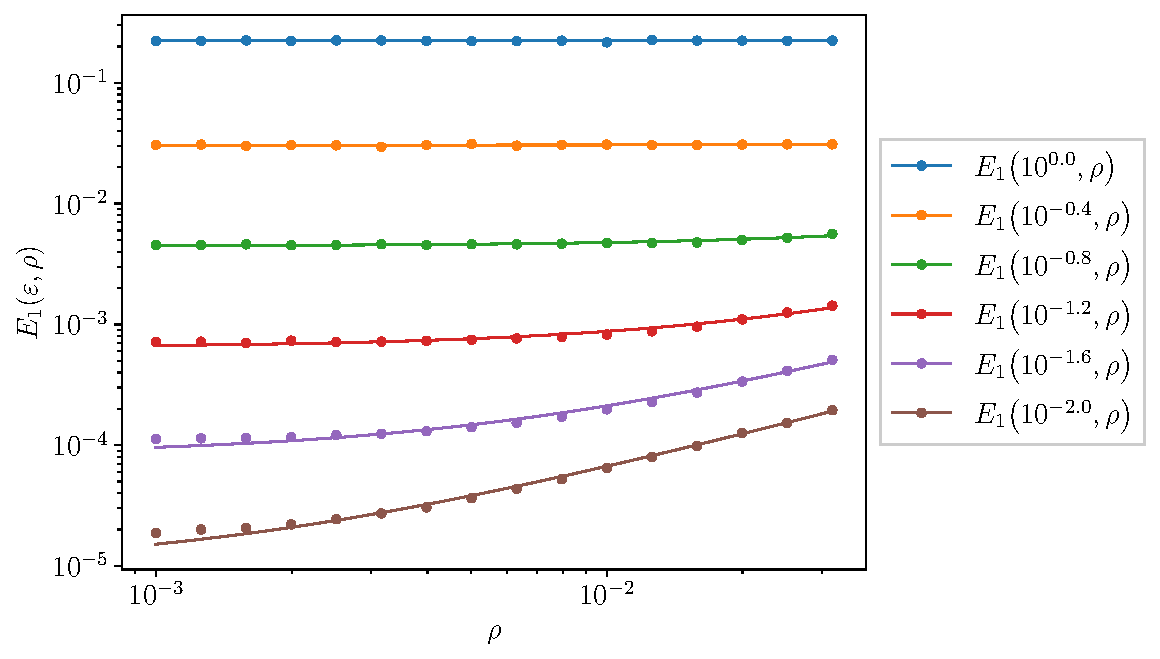
\includegraphics[width=\textwidth]{chp04_paper_numerics/figures/multiplicative/str_err_rho_r_1.0_log.pdf}
			\caption{Estimates of the strong order (with \(r = 1\)) for varying initial uncertainty parameter \(\rho\).
				Each colour corresponds to a different value of the ongoing uncertainty parameter \(\epsilon\).
				A (least squares) line of best fit of the form \(\beta_0 + \beta_1 \rho\) is included in the corresponding colour.}
			\label{fig:multiplicative_delta_lines}
		\end{subfigure}
		\caption{Validation of the theoretical bound predicted by \Cref{thm:main}, when \(r = 1\), on numerical realisations of the solution to the 1D example \cref{eqn:1d_mult}.}
		\label{fig:multiplicative_delta_eps_lines}
	\end{center}
\end{figure}

\subsection{Fixed initial condition}\label{sec:numerics_2d}
In this example, we consider a two-dimensional model and a fixed initial condition, to validate the results presented in \Cref{sec:theory_fixed}.
Following the example in Chapter 5 of \citet{SamelsonWiggins_2006_LagrangianTransportGeophysical}, we consider an unsteady meandering jet in two dimensions, which may serve as an idealised model of geophysical Rossby waves \citep{Pierrehumbert_1991_ChaoticMixingTracer}.
The velocity field for \(y \equiv \left(y_1, y_2\right)^{\T}\) is given by
\begin{equation}
	u\!\left(y, t\right) = \begin{bmatrix}
		c - A\sin\!\left(Ky_1\right)\cos\!\left(y_2\right) + \oldepsilon_{\mathrm{mj}} l_1\sin\!\left(k_1\left(y_1 - c_1 t\right)\right)\cos\!\left(l_1 y_2\right) \\
		AK\cos\!\left(Ky_1\right)\sin\!\left(y_2\right) + \oldepsilon_{\mathrm{mj}} k_1\cos\!\left(k_1\left(y_1 - c_1t\right)\right)\sin\!\left(l_1 y_2\right)
	\end{bmatrix}.
	\label{eqn:jet_ex}
\end{equation}
The velocity field describes a kinematic travelling wave with deterministic oscillatory perturbations in a co-moving frame.
Here, \(A\) is the amplitude and \(c\) is the phase speed of the primary wave, and \(K\) is the wavenumber in the \(y_1\)-direction.
The oscillatory perturbation has amplitude \(\oldepsilon_{\mathrm{mj}}\), phase speed \(c_1\) (in the co-moving frame), and wavenumbers \(k_1\) and \(l_1\) in the \(y_1\)- and \(y_2\)-directions respectively.
Throughout, we take the parameter values \(c = 0.5\), \(A = 1\), \(K = 4\), \(l_1 = 2\), \(k_1 = 1\), \(c_1 = \pi\), and \(\oldepsilon_{\mathrm{mj}} = 0.3\).
For these values, the flow consists of a meandering jet with vortex structures within the meanders, and a chaotic zone which influences the fluid transfer between the jet and the vortices.

We introduce multiplicative noise by considering stochastic perturbations to the phase speed \(c\) and the primary amplitude \(A\), which we model with the respective components of a \(2\)-dimensional Wiener process \(W_t = \left(W_t^{(1)}, W_t^{(2)}\right)^{\T}\).
Then, we specify the diffusion term as
\begin{equation}
	\sigma\!\left(y,t\right) = \begin{bmatrix}
		1 & \sin\!\left(Ky_1\right)\cos\!\left(y_2\right)  \\
		0 & K\cos\!\left(Ky_1\right)\sin\!\left(y_2\right)
	\end{bmatrix}.
	\label{eqn:jet_ex_sigma}
\end{equation}


We consider the fixed initial condition \(x_0 = \left(0, 1\right)\) and the prediction of the model at time \(t = 1\).
We then consider a linearisation of the SDE about the deterministic trajectory \(F_0^t\!\left(x_0\right)\), where \(F_0^t\) is the deterministic flow map corresponding to the vector field \cref{eqn:jet_ex}.
To compute the Gaussian distribution \cref{eqn:linear_gauss_sol} of the linearised solution, we again solve \cref{eqn:pi_ode} numerically with initial condition \(\Sigma_0^t\!\left(x_0\right) = O\).
Specifically, \cref{eqn:pi_ode} is solved jointly with the deterministic state equation \cref{eqn:ode_det} using the hybrid method proposed by \citet{Mazzoni_2008_ComputationalAspectsContinuous}.
This hybrid method combines a Taylor-Heun approximation with a Gauss-Legendre one and ensures that the numerical solution of the covariance equation is symmetric and positive semi-definite while maintaining both accuracy and computational efficiency.


\Cref{fig:y_hists} shows the resulting simulations of \(y_t^{(\epsilon)}\) for four different values of \(\epsilon\).
The realisations are binned as a histogram and bin counts are normalised, to provide an empirical estimate of the probability density function of \(y_t^{(\epsilon)}\).
Superimposed (in solid black) are the first, second and third standard-deviation contours of the probability density function of the Gaussian distribution that solves the linearised equation.
The first three standard-deviation levels of the \(2\times 2\) sample covariance matrix of the realisations of \(y_t^{(\epsilon)}\), are also overlaid (in dashed blue).
As \(\epsilon\) decreases towards \(0\), the samples increasingly resemble a Gaussian distribution, and both the mean and covariance coincide with the corresponding limits.

\begin{figure}
	\begin{center}
		\begin{subfigure}{0.49\textwidth}
			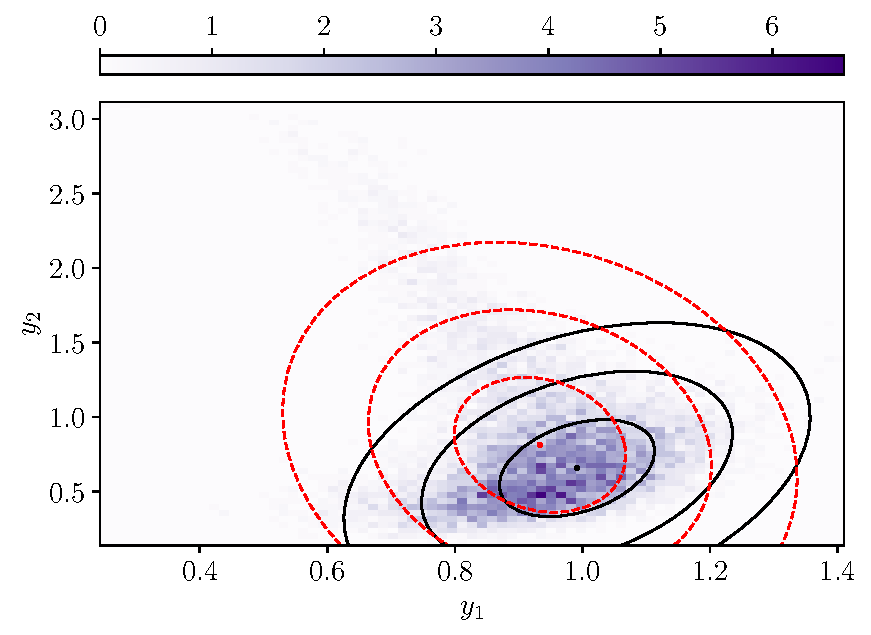
\includegraphics[width=\textwidth]{chp04_paper_numerics/figures/rossby/hist_0.1.pdf}
			\caption{\(\epsilon = 10^{-1}\)}
			\label{fig:y_hists_a}
		\end{subfigure}
		\begin{subfigure}{0.49\textwidth}
			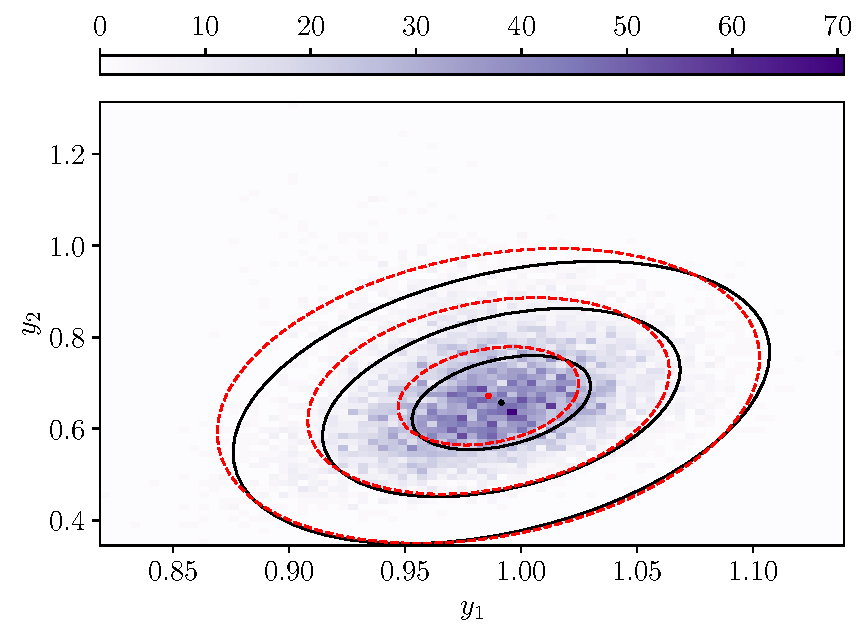
\includegraphics[width=\textwidth]{chp04_paper_numerics/figures/rossby/hist_0.03162277660168379.pdf}
			\caption{\(\epsilon = 10^{-1.5}\)}
			\label{fig:y_hists_b}
		\end{subfigure}
		\begin{subfigure}{0.49\textwidth}
			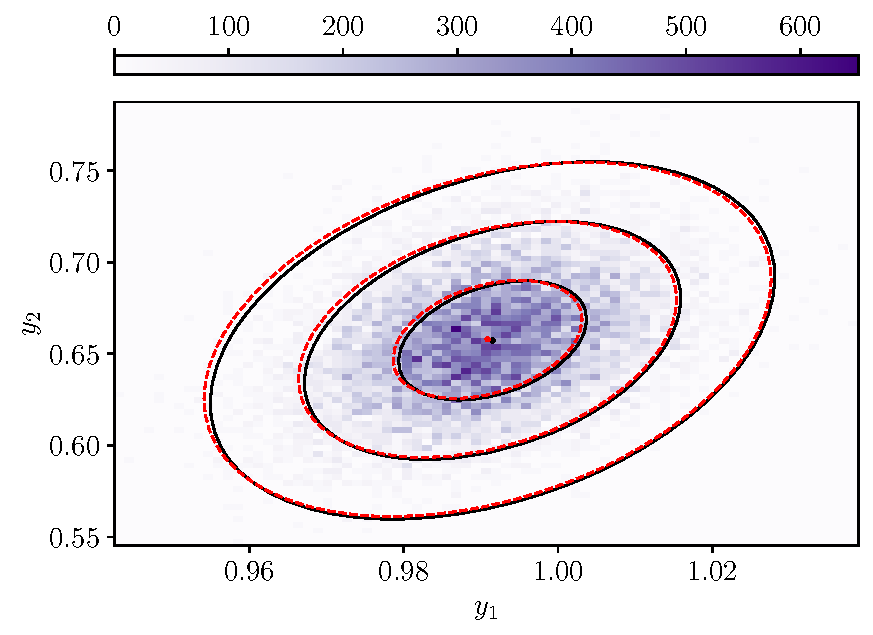
\includegraphics[width=\textwidth]{chp04_paper_numerics/figures/rossby/hist_0.010000000000000002.pdf}
			\caption{\(\epsilon = 10^{-2}\)}
			\label{fig:y_hists_c}
		\end{subfigure}
		\begin{subfigure}{0.49\textwidth}
			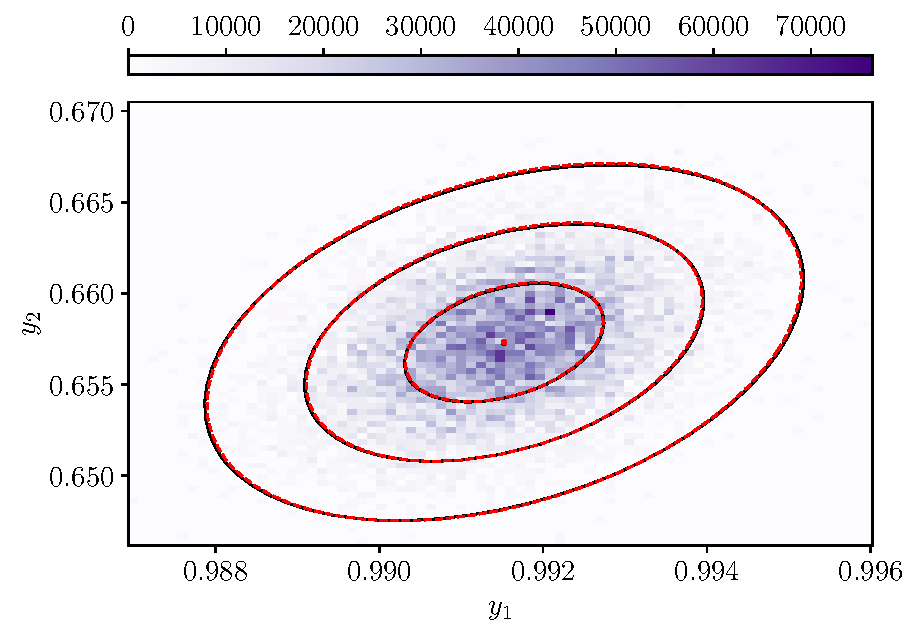
\includegraphics[width=\textwidth]{chp04_paper_numerics/figures/rossby/hist_0.001.pdf}
			\caption{\(\epsilon = 10^{-3}\)}
			\label{fig:y_hists_d}
		\end{subfigure}
		\caption{Histograms of \(y_t^{(\epsilon)}\) from direct simulation of the SDE with drift \cref{eqn:jet_ex} and diffusivity \cref{eqn:jet_ex_sigma} subject to the fixed initial condition, for four different \(\epsilon\) values.
		Overlaid in black are contours of the Gaussian solution \cref{eqn:linear_gauss_sol} of the linearised SDE \cref{eqn:linear_sde_inform}, which correspond to the first three standard deviation levels centred at the mean \(F_0^t(x)\).
		In dashed blue are corresponding contours computed from the sample covariance matrix of the realisations.
		}
		\label{fig:y_hists}
	\end{center}
\end{figure}

For a fixed initial condition, \cref{eqn:main_ineq} predicts that the expected distance between the original SDE solution and that of a linearisation satisfies
\[
	\avg{\norm{y_t^{(\epsilon)} - l_t^{(\epsilon)}}^r} \leq \left(K_{\nabla\nabla u} + K_{\nabla\sigma}\right)D_1\!\left(r,t, K_{\nabla u}, K_\sigma\right)\epsilon^{2r}.
\]
To numerically estimate the left-hand side of \cref{eqn:main_ineq}, we again use a Monte-Carlo estimator;
\[
	E_r\!\left(\epsilon\right) \coloneqq \frac{1}{N}\sum_{i=1}^N{\norm{\hat{y}_i^{(\epsilon)} - \hat{l}_i^{(\epsilon)}}^r}.
\]
For \(r = 1,2,3,4\), \(E_r\!\left(\epsilon\right)\) is shown (in a logarithmic scale) for decreasing values of \(\epsilon\) in \Cref{fig:gamma_z_valid}.
\Cref{thm:main} predicts that \(\log_{10}\left(E_r\!\left(\epsilon\right)\right)\) should decay linearly with a slope greater than \(2r\) as \(\epsilon\) decreases to zero.
The least squares lines of best fit for each value of \(r\) in \Cref{fig:gamma_z_valid} show this behaviour, and are therefore consistent with \Cref{thm:main}.

\begin{figure}
	\begin{center}
		\begin{subfigure}{0.49\textwidth}
			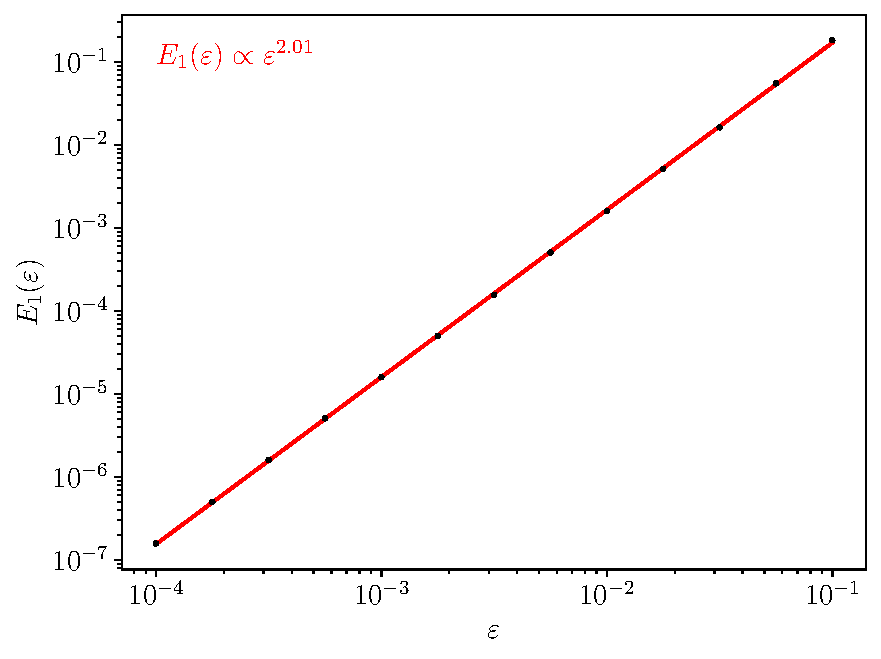
\includegraphics[width=\textwidth]{chp04_paper_numerics/figures/rossby/str_err_r_1.0.pdf}
			\caption{\(r = 1\) (mean)}
			\label{fig:gamma_z_valid_1}
		\end{subfigure}
		\begin{subfigure}{0.49\textwidth}
			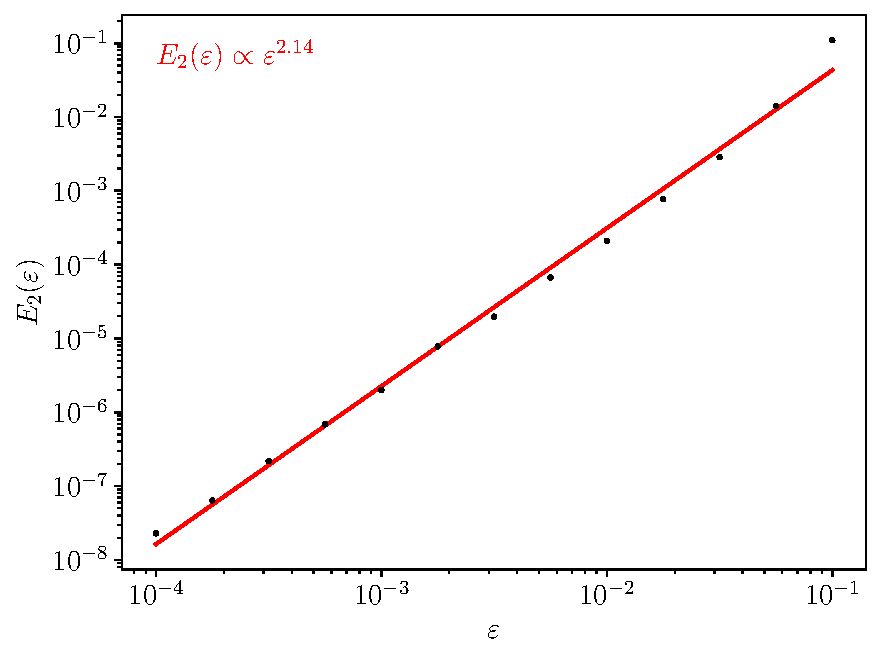
\includegraphics[width=\textwidth]{chp04_paper_numerics/figures/rossby/str_err_r_2.0.pdf}
			\caption{\(r = 2\) (variance)}
			\label{fig:gamma_z_valid_2}
		\end{subfigure}
		\begin{subfigure}{0.49\textwidth}
			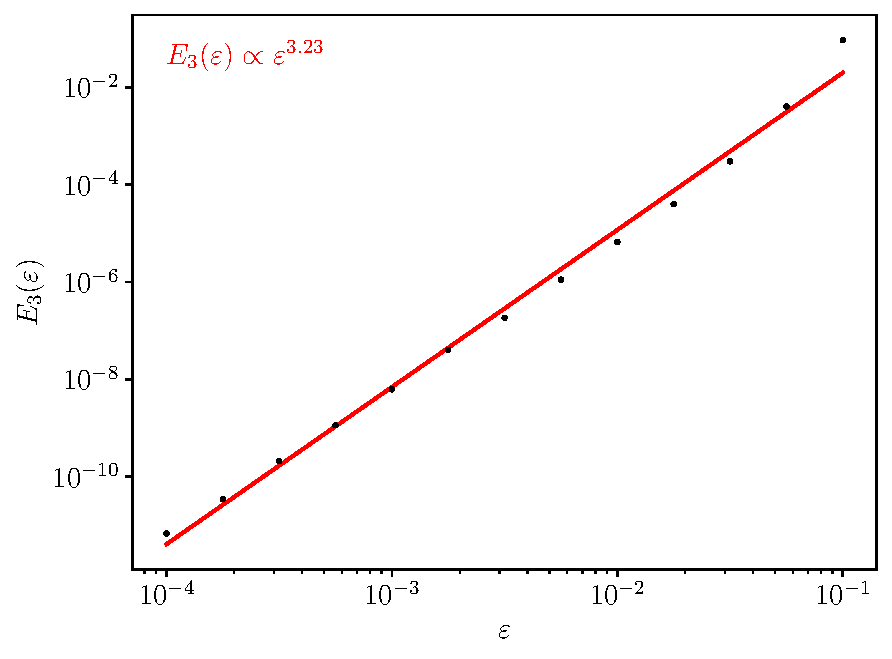
\includegraphics[width=\textwidth]{chp04_paper_numerics/figures/rossby/str_err_r_3.0.pdf}
			\caption{\(r = 3\) (skewness)}
			\label{fig:gamma_z_valid_3}
		\end{subfigure}
		\begin{subfigure}{0.49\textwidth}
			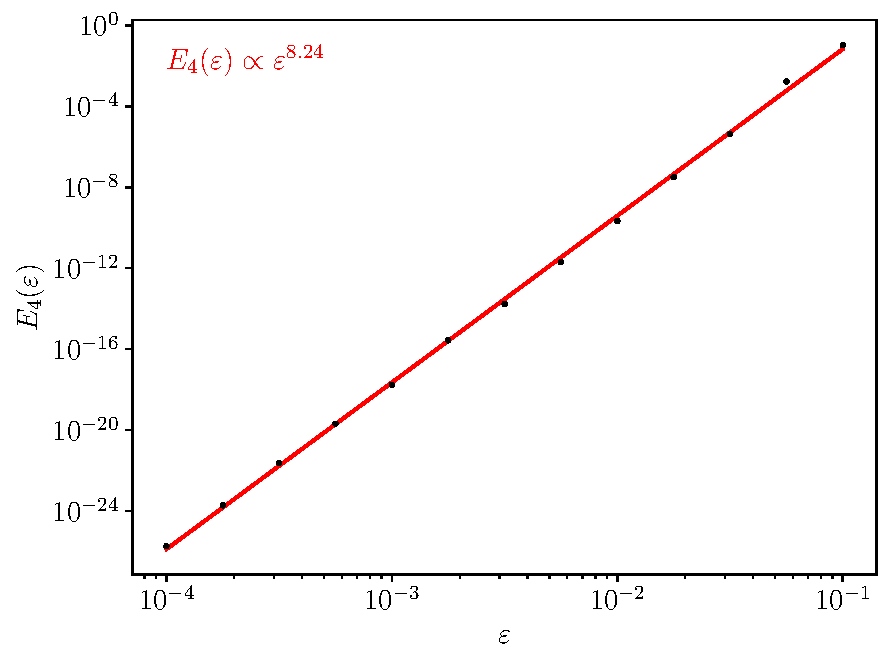
\includegraphics[width=\textwidth]{chp04_paper_numerics/figures/rossby/str_err_r_4.0.pdf}
			\caption{\(r = 4\) (kurtosis)}
			\label{fig:gamma_z_valid_4}
		\end{subfigure}

		\caption{Validation of \Cref{thm:main}, by plotting the sample \(r\)th raw moment distance (the error metric \(E_r(\epsilon)\)) between \(10000\) realisations of the meandering jet SDE and a corresponding linearisation, for decreasing values of \(\epsilon\).
			A line of best fit (in red) is placed on each, and the resulting slope indicated.}
		\label{fig:gamma_z_valid}
	\end{center}
\end{figure}


\section{Computing stochastic sensitivity} \label{sec:comput_s2}
In this section, we illustrate the computability of stochastic sensitivity as described in \Cref{thm:s2_calculation}.
We again consider the meandering jet \cref{eqn:jet_ex} with multiplicative noise described by \cref{eqn:jet_ex_sigma}.
We take the same choice of parameters as in \cref{sec:numerics_2d}, except for the perturbation amplitude \(\oldepsilon_{\mathrm{mj}}\) which is varied to obtain qualitatively different behaviour in the system.
For each initial condition in a \(400 \times 400\) uniform grid on \(\left[0, \pi\right] \times \left[0, \pi\right]\), the \(S^2\) value is calculated using \cref{eqn:s2_calculation}.
\Cref{fig:ex_jet_s2_field} shows the resulting \(S^2\) field from time \(0\) to \(t = 1\), for two different values of \(\oldepsilon_{\mathrm{mj}}\).

\begin{figure}
	\begin{center}
		\begin{subfigure}{0.49\textwidth}
			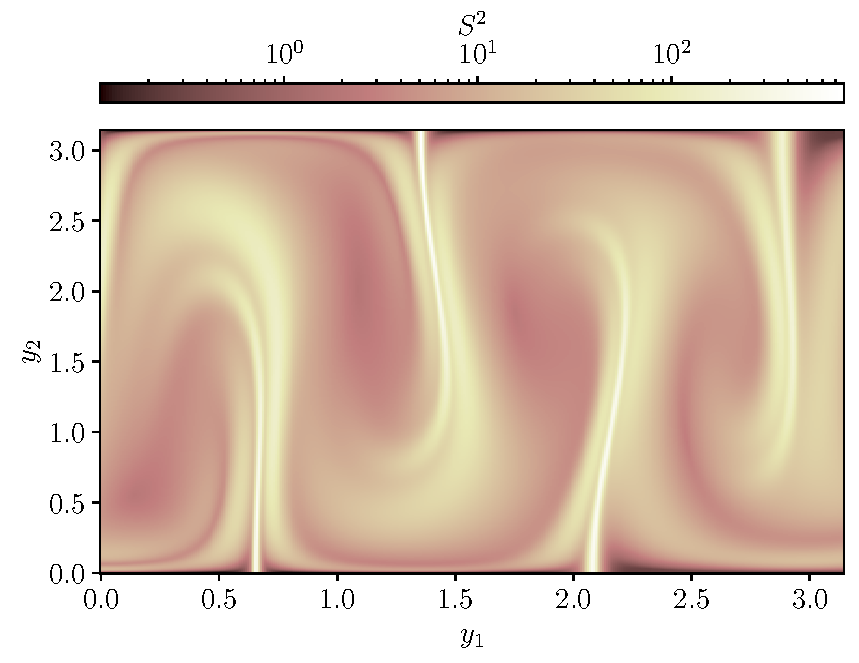
\includegraphics[width=\textwidth]{chp04_paper_numerics/figures/rossby/S2_zero_0.3.pdf}
			\caption{\(\oldepsilon_{\mathrm{mj}} = 0.3\)}
			\label{fig:s2_field_0.3}
		\end{subfigure}
		\begin{subfigure}{0.49\textwidth}
			\includegraphics[width=\textwidth]{chp04_paper_numerics/figures/rossby/s2_zero_1.0.pdf}
			\caption{\(\oldepsilon_{\mathrm{mj}} = 1.0\)}
			\label{fig:s2_field_1.0}
		\end{subfigure}
		% \includegraphics[width=\textwidth]{figures/s2_field_0.3.pdf}
		\caption{The \(S^2\) field of the meandering jet flow \cref{eqn:jet_ex} over the time interval \([0,1]\), for two different sets of parameters with qualitatively different behaviour.
			The \(S^2\) value for each initial condition is computed directly as the operator norm of the covariance matrix \(\Sigma_0^1\!\left(x_0\right)\), as per \cref{eqn:s2_calculation}.}
		\label{fig:ex_jet_s2_field}
	\end{center}
\end{figure}


When \(\oldepsilon_{\mathrm{mj}} = 0.3\) (\Cref{fig:s2_field_0.3}), the \(S^2\) field is largest in the elongated gyre regions outside of the meandering jet, where the flow exhibits chaotic behaviour \citep{Pierrehumbert_1991_ChaoticMixingTracer} and we accordingly expect larger uncertainty due to the model dynamics.
As a region of small \(S^2\) value, the meandering jet emerges as a coherent structure, consisting of initial points whose eventual fate is significantly more certain than in other regions.
When \(\oldepsilon_{\mathrm{mj}} = 1.0\) (\Cref{fig:s2_field_1.0}, the deterministic flow is dominated by oscillatory perturbation, which

The stochastic sensitivity field can highlight Lagrangian coherent structures within the flow, by identifying regions of the flow with a relatively small uncertainty, as measured by a \emph{single} number for each initial condition.
Subsets of the spatial domain corresponding to coherent structures can be extracted, e.g. by taking a threshold on \(S^2\) as described in the original work \citep{Balasuriya_2020_StochasticSensitivityComputable}; further examples of coherent structure extraction with stochastic sensitivity on both toy models and real data can be found in \citet{Balasuriya_2020_StochasticSensitivityComputable} and \citet{BadzaEtAl_2023_HowSensitiveAre}.
Here, we demonstrate the extraction of coherent structures.


\td{Use cyan for robust sets, to be consistent with later results.}
\begin{figure}
	\begin{center}
		\begin{subfigure}{0.49\textwidth}
			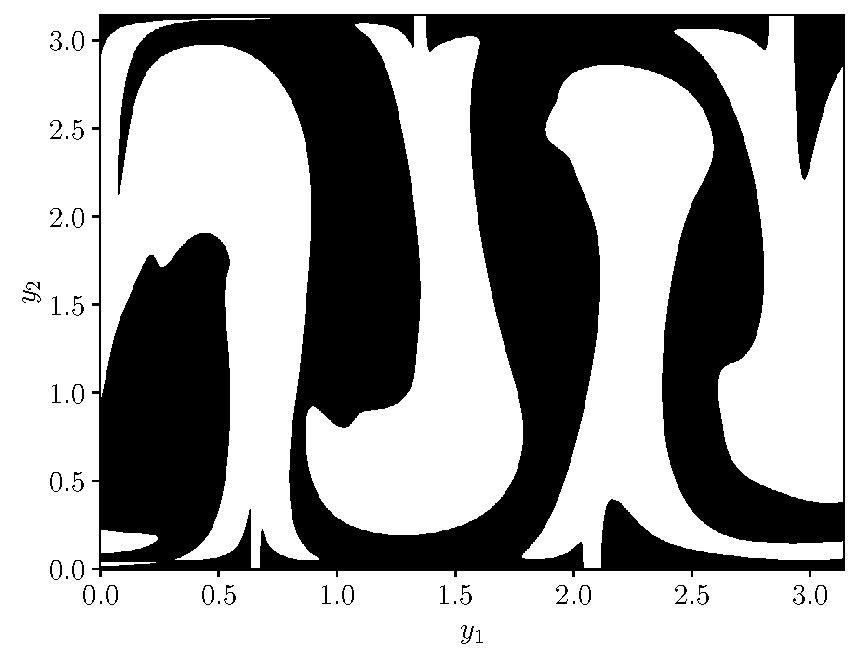
\includegraphics[width=\textwidth]{chp04_paper_numerics/figures/rossby/S2_robust_0.3.pdf}
			\caption{\(\oldepsilon_{\mathrm{mj}} = 0.3\), \(R = 10\)}
		\end{subfigure}
		\begin{subfigure}{0.49\textwidth}
			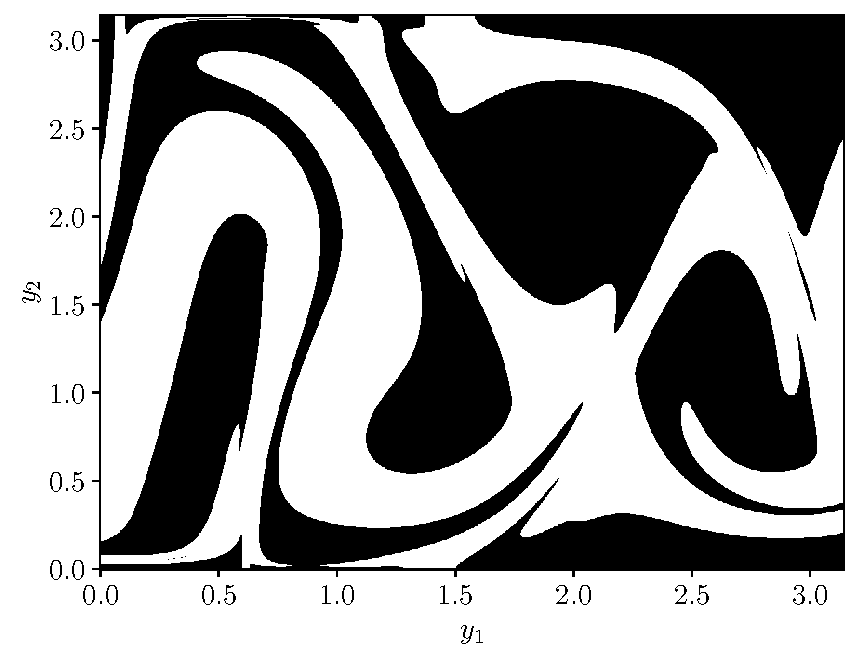
\includegraphics[width=\textwidth]{chp04_paper_numerics/figures/rossby/S2_robust_1.0.pdf}
			\caption{\(\oldepsilon_{\mathrm{mj}} = 1.0\), \(R = 10\)}
		\end{subfigure}
		\caption{Robust sets extracted from the stochastic sensitivity fields in \Cref{fig:s2_field}, by taking the initial conditions with a stochastic sensitivity value above a specified threshold \(R\). }
		\label{fig:ex_jet_robust}
	\end{center}
\end{figure}



% \begin{figure}
% 	\begin{center}
% 		\begin{subfigure}{0.49\textwidth}
% 			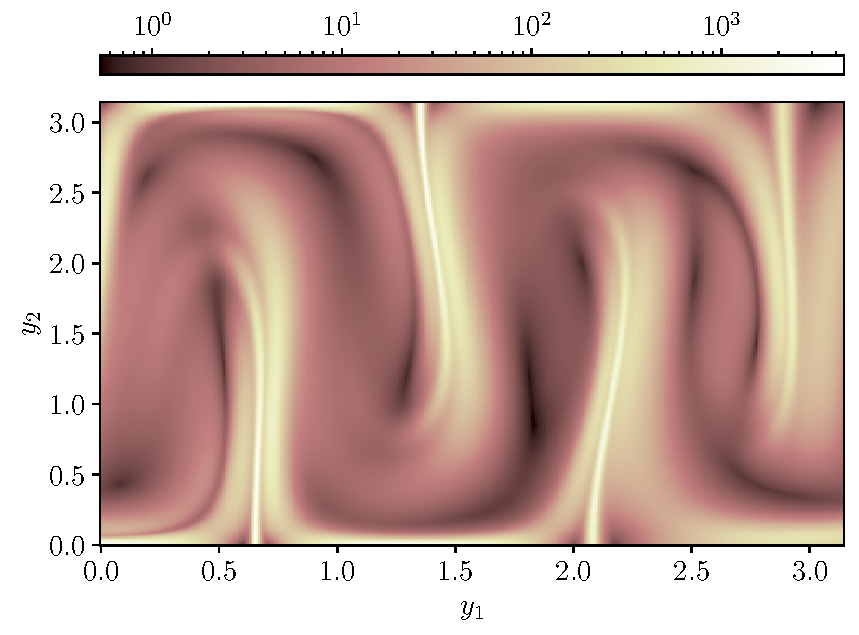
\includegraphics[width=\textwidth]{chp04_paper_numerics/figures/rossby/ftle_0.3.pdf}
% 			\caption{\(\oldepsilon_{\mathrm{mj}} = 0.3\)}
% 		\end{subfigure}
% 		\begin{subfigure}{0.49\textwidth}
% 			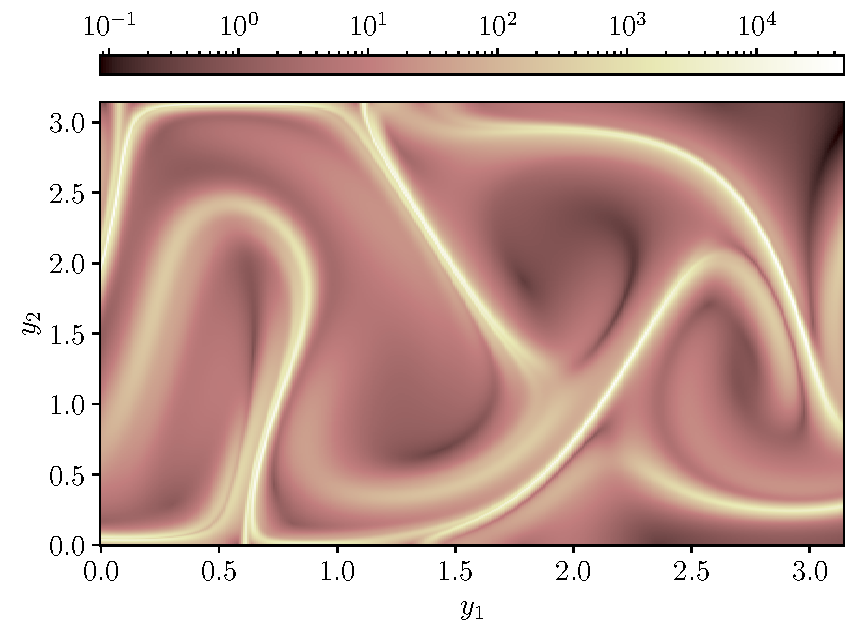
\includegraphics[width=\textwidth]{chp04_paper_numerics/figures/rossby/ftle_1.0.pdf}
% 			\caption{\(\oldepsilon_{\mathrm{mj}} = 1.0\)}
% 		\end{subfigure}
% 		\caption{The finite-time Lyapunov exponent field of the meandering jet flow \cref{eqn:jet_ex} over the time \([0,1]\), for two different values of \(\oldepsilon_{\mathrm{mj}}\).
% 			These fields should be compared with the corresponding stochastic sensitivity fields in \Cref{fig:ex_jet_s2_field}.}
% 	\end{center}
% 	\label{fig:ex_jet_ftle}
% \end{figure}



% In this example, the stochastic sensitivity and FTLE fields show strong similarities, supporting the claims in \Cref{sec:ftle_s2_connection} that stochastic sensitivity can be considered a generalisation of the FTLE.
% The two fields are quantifying different aspects of the flow, however, and so can show differences; such examples are available in \citet{Balasuriya_2020_StochasticSensitivityComputable} (see Figure 3.7) and \citet{BadzaEtAl_2023_HowSensitiveAre} (compare Figures 1 and 5, and Figures 11 and 15).

% To highlight the differences between the stochastic sensitivity field and the finite-time Lyapunov exponent, here we provide a brief and contrived example in which multiplicative noise has a substantial impact on the dynamical behaviour of the system.
% Following the example of \citet{BalasuriyaGottwald_2018_EstimatingStableUnstable}, consider the two-dimensional velocity field
% \begin{equation*}
% 	u\!\left(y, t\right) = \begin{bmatrix}
% 		-4y_1 + y_1^2 \\
% 		3y_2 - y_2^3
% 	\end{bmatrix},
% \end{equation*}
% To introduce multiplicative noise, we take the diffusivity
% \[
% 	\sigma\!\left(y,t\right) = \begin{bmatrix}
% 		1       & 0                                       \\
% 		y_2 - 1 & 3\sin\!\left(2\pi y_1\right)e^{-0.8y_1}
% 	\end{bmatrix},
% \]
% which in particular ensures a non-trivial spatial dependence along the stable manifold of interest.





% \begin{figure}
% 	\begin{center}
% 		\begin{subfigure}{0.49\textwidth}
% 			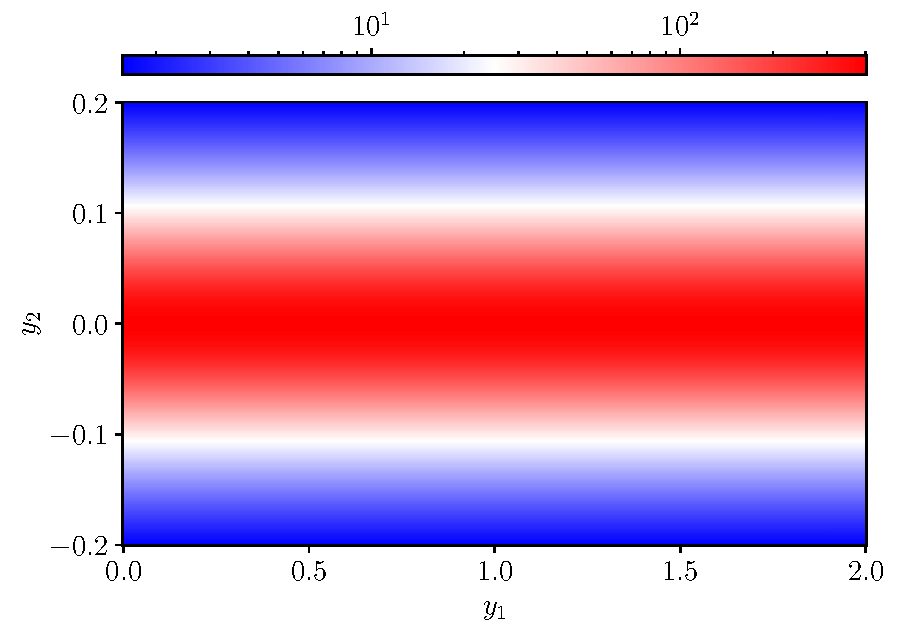
\includegraphics[width=\textwidth]{chp04_paper_numerics/figures/unstable/ftle.pdf}
% 			\caption{FTLE}
% 			\label{fig:s2_ftle_ftle}
% 		\end{subfigure}
% 		\begin{subfigure}{0.49\textwidth}
% 			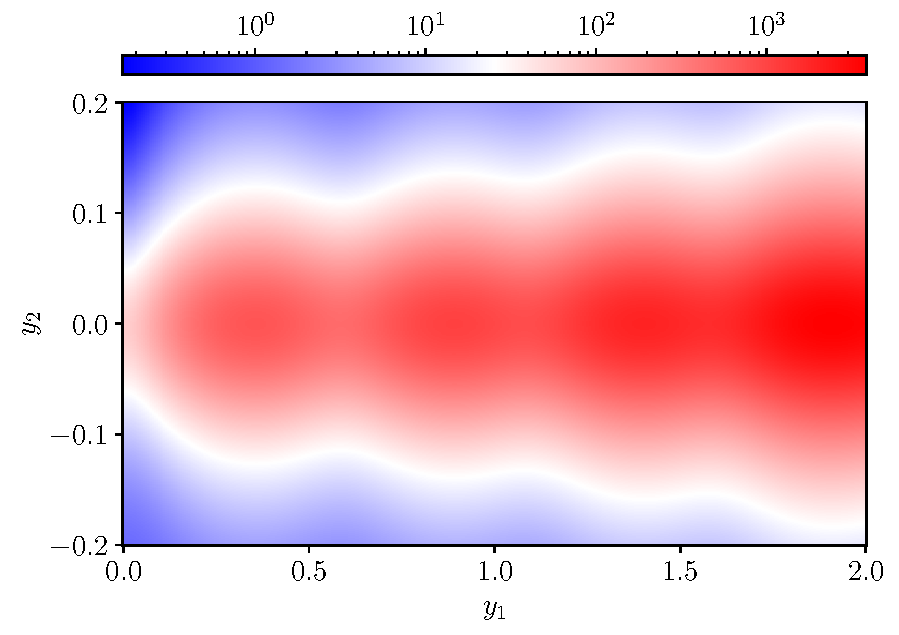
\includegraphics[width=\textwidth]{chp04_paper_numerics/figures/unstable/S2_zero.pdf}
% 			\caption{\(S^2\) with fixed initial condition.}
% 			\label{fig:s2_ftle_ftle}
% 		\end{subfigure}		\begin{subfigure}{0.49\textwidth}
% 			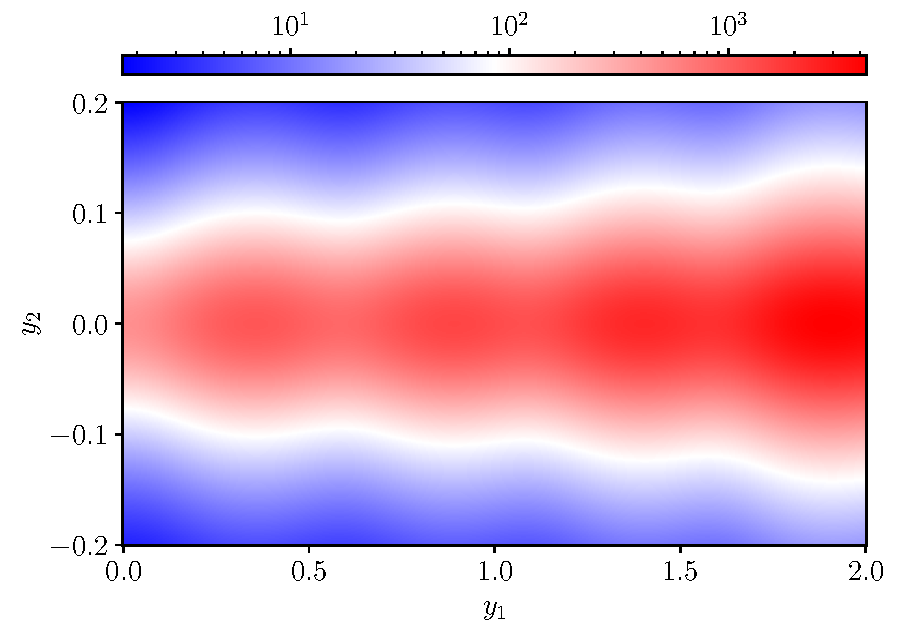
\includegraphics[width=\textwidth]{chp04_paper_numerics/figures/unstable/S2_I.pdf}
% 			\caption{\(S^2\) with standard Gaussian initial condition.}
% 			\label{fig:s2_ftle_ftle}
% 		\end{subfigure}
% 		\caption{The stochastic sensitivity and FTLE-type stretching fields for the two-dimensional}
% 		\label{fig:}
% 	\end{center}
% \end{figure}



%To briefly demonstrate that the stochastic sensitivity field and the resulting robust sets are in fact accounting for uncertainty, we consider a simpler, contrived example.
%We again take the velocity field \eqref{eqn:jet_ex} describing the meandering jet, but now assume that the ongoing stochasticity is 1-dimensional, i.e. \(m = 1\) in the notation of \Cref{ch:linear_theory}, and only acts on the \(y_1\)-component.
%That is, we are considering the stochastic model
%\[
%	\dif \begin{bmatrix}
%		y_1 \\ y_2
%	\end{bmatrix} = u\!\left(\begin{bmatrix}
%			y_1 \\ y_2
%		\end{bmatrix}, t\right)\dif t + \epsilon \begin{bmatrix}
%		S y_1 \\  0
%	\end{bmatrix} \dif W_t
%\]
%where \(W_t\) is a one-dimensional Wiener process, and \(S\) is a large constant.
%Intuitively, one would expect that the large uncertainty in the \(y_1\)-direction will result in a `smearing out' of trajectories in that direction and therefore a loss of coherence of the jet structure
%We illustrate this by computing the stochastic sensitivity field, and plotting this in \Cref{fig:jet_ex_y1_only} alongside the finite-time Lyapunov field over the same spatiotemporal region.

%\begin{figure}
%	\begin{center}
%		%
%		\begin{subfigure}{0.49\textwidth}
%			\caption{}
%		\end{subfigure}
%		\begin{subfigure}{0.49\textwidth}
%			\caption{}
%		\end{subfigure}
%		\caption{}
%		\label{fig:jet_ex_y1_only}
%	\end{center}
%\end{figure}


%This was a contrived example, but demonstrates that the stochastic sensitivity field provides further insight into the qualitative behaviour of

%Moreover, this simple example demonstrates the claim in \Cref{sec:theory_s2} that the stochastic sensitivity field can be considered a generalisation of the finite-time Lyapunov exponent, in that features of the latter are captured while additionally accounting for ongoing uncertainties.
